\chapter{Experimental Evaluation}
\label{ch:evaluation}
\chaptermark{Experimental Evaluation}

This chapter reports the evidence for the four research questions.
\Cref{sec:7-2} compares JHQ-GPU with other GPU indexes (RQ4);
\cref{sec:7-3,sec:7-4,sec:7-6} evaluate representation-aware execution
and its selection correctness (RQ2); \cref{sec:7-5} tests workload-level
refinement calibration (RQ3); and \cref{sec:7-7} measures GPU construction
and capacity (RQ1). \Cref{sec:7-8} examines numerical sensitivity and
what can be attributed to each source of recall loss.

\section{Experimental Protocol}
\label{sec:7-1}

\subsection{Comparison protocol and reproducibility}

The comparisons use the datasets, host-to-host timing and frontier rules
in \cref{sec:3-2,sec:3-3,sec:3-4}. Search throughput excludes construction
and calibration; each execution ablation retains its own baseline.
\Cref{tab:3-campaigns,tab:a-components} identify experiment families,
implementations and result locations, while \cref{sec:a-e1-protocol}
records timing conventions. Supplementary tests are distinguished below
by whether their baselines were measured alongside JHQ or taken from
the main comparison. The historical CPU result is reported separately
in \cref{sec:7-cpu}.

\section{Cross-System Recall--Throughput Comparison}
\label{sec:7-2}

\subsection{Comparison scope and frontier construction}

At recall 0.97 and batch 1,000, JHQ-GPU leads the tested methods on
Vogue and both OpenAI datasets, nearly ties IVF-RaBitQ on arXiv, and
delivers $1.32$--$1.75\times$ CAGRA fp32 throughput across all four
(\cref{fig:7-frontiers,tab:7-matched}). The main comparison uses the first four datasets in
\cref{tab:3-data}, common queries and ground truth, and the graph,
compressed-IVF and brute-force baselines of \cref{sec:3-4}
\cite{cagra,pq,ivfrabitq}. Its 1,590 valid measurements cover 27--39 JHQ
configurations per dataset and 54--264 per baseline family. The finite
parameter coverage is recorded in \cref{tab:3-grids,sec:b-grids}.

Execution differs by workload. All 105 arXiv and OpenAI configurations
use one block per query ($\gscan=0$); the 27 Vogue configurations use
four groups ($\gscan=4$), triggered by candidate-count coefficients of
variation between 0.338 and 0.622. Thus only Vogue's frontier includes
grouped retention, shared bounds and merging (\cref{sec:5-5}).

The frontiers also compare different storage budgets. Nine-bit RaBitQ
has the same nominal $9d/8$ code bytes per vector as JHQ, while its
four- and eight-bit variants use less. \Cref{tab:4-bytes,sec:7-7}
report representation costs and measured allocations alongside speed.

\begin{figure}[!htbp]
\centering
\includegraphics[width=\linewidth]{ch7/frontiers.pdf}
\caption[Main-comparison recall--throughput frontiers]{Measured host-to-host recall--QPS frontiers on the four main-comparison datasets.
The displayed recall window begins at 0.90, with a vertical line at 0.97;
all baseline families,
including CAGRA int8, participate in frontier construction. Lines connect
measured points; throughput uses a logarithmic axis.}
\label{fig:7-frontiers}
\end{figure}

\subsection{Throughput at matched recall}

The lead over CAGRA fp32 holds under both estimators, while the much
smaller arXiv--RaBitQ margin changes direction
(\cref{tab:7-matched}). The interpolated and qualifying-measured
estimators follow \cref{sec:3-4}.

\par\medskip\noindent\begin{minipage}{\linewidth}
\captionsetup{hypcap=false}
\centering
\captionof{table}[Cross-system comparison at recall 0.97]{Recall 0.97 comparison. Each ratio is interpolated / measured;
values above one favour JHQ. JHQ kQPS is the interpolated estimate.
The small arXiv--RaBitQ difference changes direction with the estimator.}
\label{tab:7-matched}
\small\setlength{\tabcolsep}{4pt}
% Generated by scripts/build_ch7.py; do not edit numbers manually.
\begin{tabular}{@{}lrrr@{}}
\toprule
Dataset & JHQ kQPS & vs CAGRA fp32 & vs IVF-RaBitQ \\
\midrule
Vogue & 230.8 & 1.416 / 1.537 & 1.059 / 1.046 \\
arXiv & 258.6 & 1.317 / 1.422 & 0.996 / 1.015 \\
OpenAI-1536 & 126.7 & 1.747 / 2.294 & 1.130 / 1.111 \\
OpenAI-3072 & 55.9 & 1.747 / 2.088 & 1.157 / 1.346 \\
\bottomrule
\end{tabular}

\end{minipage}\par\medskip

Vogue's modest RaBitQ lead depends on grouped execution. At fixed
index, probes, budget and final outputs, replacing the grouped path by
one block lowers the recall-0.97 JHQ/RaBitQ ratio from 1.059 to 0.933
at batch 1,000. CAGRA int8 is $1.20$--$1.98\times$ faster at recall
0.90--0.92 but cannot reach 0.97 within its tested grid. RaBitQ leads
at some targets above 0.98, and CAGRA fp32 leads near 0.99 on arXiv
(\cref{fig:7-frontiers}).

\subsection{Precision sensitivity on the OpenAI datasets}
\label{sec:7-precision}

Using FP32 in place of TF32 reduces throughput by about 5\% at matched
configurations, while the checked FP32 frontiers retain their lead over
CAGRA fp32. Source inspection found that the main implementation uses
TF32 multiplication with FP32 accumulation for OpenAI rotation and
centroid matrix products (\cref{sec:4-2}). The precision check
changes that arithmetic switch and alternates the two variants across
probe settings: 37 OpenAI-1536 and 39 OpenAI-3072 configurations, five
rounds each at batch 1,000. Both reuse one TF32-trained model; add and
query arithmetic, including encoding and routing, change. This is not
independent FP32 retraining.

\par\medskip\noindent\begin{minipage}{\linewidth}
\centering\captionsetup{hypcap=false}
\captionof{table}[FP32 sensitivity at matched configurations]{FP32 sensitivity. QPS ratio is FP32/TF32 at equal configuration
(geometric mean); recall differences have the same direction. The last
two columns compare the FP32 frontier at recall 0.97 with archived
IVF-RaBitQ and CAGRA fp32 frontiers. The precision check reuses baseline measurements from the main comparison.}
\label{tab:7-precision}
\scriptsize\setlength{\tabcolsep}{3pt}
\begin{tabular}{@{}lrrrrr@{}}
\toprule
Dataset & Pairs & QPS ratio & $\Delta$Recall & vs RaBitQ & vs CAGRA \\
\midrule
OpenAI-1536 & 37 & 0.953 & +0.0003--+0.0005 & 1.086 & 1.679 \\
OpenAI-3072 & 39 & 0.951 & +0.0000--+0.0003 & 1.079 & 1.629 \\
\bottomrule
\end{tabular}

\end{minipage}\par\medskip

At matched configuration, recall increases by 0--0.0005. At recall 0.97,
FP32 is about 3\% slower than TF32 measured alongside it, but its ratios
to archived RaBitQ are 1.086 on OpenAI-1536 and 1.079 on OpenAI-3072;
ratios to archived CAGRA fp32 are 1.679 and 1.629. The repeated original
variant gives RaBitQ ratios of 1.118 and 1.114, compared with historical
1.130 and 1.157. \Cref{fig:7-precision} shows this paired precision
comparison; the next check remeasures the baselines.

\par\medskip\noindent\begin{minipage}{\linewidth}
\captionsetup{hypcap=false}
\centering
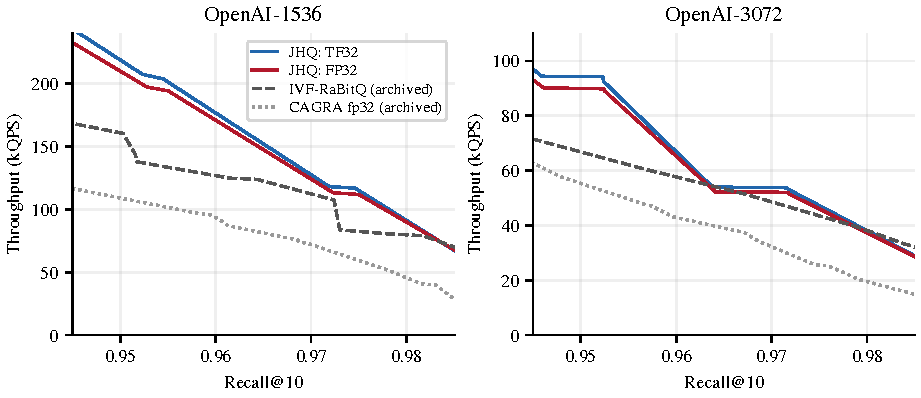
\includegraphics[width=\linewidth]{variants/final-polish/figures/precision.pdf}
\captionof{figure}[TF32 and FP32 precision frontiers]{Precision check. Solid curves are JHQ variants measured together;
dashed/dotted baselines come from the main comparison.
All use the chapter's frontier and interpolation rules.}
\label{fig:7-precision}
\end{minipage}\par\medskip

\subsection{Baselines remeasured with JHQ}
\label{sec:b-precision-anchors}

The same-session check confirms an FP32 lead at recall 0.97 under
both estimators in its tested grid. \Cref{tab:b-precision-anchors}
reports ratios to both RaBitQ and CAGRA fp32.

Twelve paired configurations per OpenAI dataset use the main
comparison's memory-pool settings. Two five-round JHQ repetitions
bracket the baseline runs, and their median rates are combined
geometrically. Equal-configuration FP32/TF32 means are 0.956 for
OpenAI-1536 and 0.964 for OpenAI-3072. Both variants reuse TF32-trained
caches and change only add/query arithmetic.

\par\medskip\noindent\begin{minipage}{\linewidth}
\captionsetup{hypcap=false}
\centering
\captionof{table}[Baselines remeasured with JHQ]{The same-session check at recall 0.97, batch 1,000. Baseline ratios are interpolation / strict measured threshold; FP32/TF32 is interpolated. All methods were remeasured together; the precision check instead reuses the main comparison's baselines.}
\label{tab:b-precision-anchors}
\footnotesize\setlength{\tabcolsep}{3pt}
\begin{tabular}{@{}lrrr@{}}
\toprule
Dataset & FP32/TF32 at 0.97 & FP32 / RaBitQ & FP32 / CAGRA \\
\midrule
OpenAI-1536 & 0.980 & 1.126 / 1.053 & 1.752 / 1.633 \\
OpenAI-3072 & 0.973 & 1.328 / 1.316 & 1.825 / 2.019 \\
\bottomrule
\end{tabular}

\end{minipage}\par\medskip

The check covers a limited grid near recall 0.97. OpenAI-3072's RaBitQ
bracket spans recall 0.9669--0.9796, so the size of the margin depends
on grid coverage and estimator. It is evidence for this local comparison,
not for independently FP32-trained frontiers or every recall target.


\subsection{Interpreting the OpenAI comparison}

The two OpenAI exports provide a useful dimension comparison because
both derive from Qdrant's DBpedia embeddings
\cite{data_openai1536,data_openai3072}. Alignment was checked before
interpreting their different widths: after truncation and
renormalisation, all 1,000 query rows and 10,299 sampled database rows
have cosine $\geq0.9980$, with median 1.000000; their ground-truth sets
share 9.046 of ten neighbours on average. These checks support row
alignment without establishing a complete original-entity-ID join.
Doubling dimension leaves the CAGRA fp32 ratio at 1.747 and changes the
RaBitQ ratio from 1.130 to 1.157, so dimension alone does not explain
the observed advantage.

At 128 probes, larger gains accompany smaller refinement multipliers:
4--8 on OpenAI, 64 on Vogue and 100 on arXiv, whose later full-pool
calibration selects 200. This is an association across workloads,
not a controlled causal comparison; \cref{sec:8-centring} tests one
representation-level explanation. Small margins and measurement
sensitivity are examined in \cref{sec:7-8}.

\subsection{Small batches change the competitive region}
\label{sec:7-smallbatch}

At batch 8 and recall 0.97, CAGRA fp32 is faster on all four datasets
under both estimators. JHQ remains competitive at lower recall, but
near ties depend on how measured endpoints are used. The small-batch
study compares scheduled JHQ, CAGRA fp32/int8 and IVF-RaBitQ at
batches 8 and 32 on the four main-comparison datasets. Five synchronous
host-to-host rounds use 1,000 and 992 queries, respectively. The
1,808 measurements include a one-block JHQ control; IVF-PQ and brute
force are outside this study.

\suppressfloats[t]
\par\medskip\noindent\begin{minipage}{\linewidth}
\captionsetup{hypcap=false}
\centering
\includegraphics[width=\linewidth]{t4-t5/smallbatch.pdf}
\captionof{figure}[Small-batch competitive regions]{Small-batch JHQ / fastest-competitor
QPS under interpolation with qualifying measured endpoints. Above one
favours JHQ. \Cref{tab:7-smallbatch} gives strict thresholds.}
\label{fig:7-smallbatch}
\end{minipage}\par\medskip

\par\medskip\noindent\begin{minipage}{\linewidth}
\captionsetup{hypcap=false}
\centering
\captionof{table}[Small-batch matched-recall ratios]{Small-batch QPS ratios:
interpolation with qualifying endpoints / strict measured threshold.
The fastest competitor is selected independently for each estimator;
higher-recall qualifying endpoints remain eligible without extrapolation.}
\label{tab:7-smallbatch}
\footnotesize\setlength{\tabcolsep}{4pt}
\begin{tabular}{@{}lrrrr@{}}
\toprule
Dataset & $b$ & $R=0.90$ & $R=0.95$ & $R=0.97$ \\
\midrule
Vogue & 8 & 1.155 / 1.091 & 1.073 / 0.980 & 0.893 / 0.854 \\
Vogue & 32 & 1.069 / 0.997 & 0.956 / 0.895 & 0.865 / 0.839 \\
arXiv & 8 & 1.479 / 1.454 & 0.859 / 0.851 & 0.697 / 0.698 \\
arXiv & 32 & 1.166 / 1.148 & 0.667 / 0.661 & 0.622 / 0.582 \\
OpenAI-1536 & 8 & 1.316 / 1.131 & 0.851 / 0.825 & 0.641 / 0.620 \\
OpenAI-1536 & 32 & 1.071 / 0.915 & 0.770 / 0.752 & 0.937 / 0.914 \\
OpenAI-3072 & 8 & 1.032 / 0.953 & 0.798 / 0.798 & 0.721 / 0.702 \\
OpenAI-3072 & 32 & 0.866 / 0.734 & 0.608 / 0.771 & 1.008 / 1.351 \\
\bottomrule
\end{tabular}

\end{minipage}\par\medskip

At recall 0.97, interpolated JHQ/fastest-competitor ratios are
0.641--0.893 for batch 8 and 0.622--1.008 for batch 32.
OpenAI-3072 favours JHQ under the batch-32 measured threshold, while
Vogue's batch-8 lead at recall 0.95 requires interpolation
(\cref{tab:7-smallbatch}).

At recall 0.90, interpolation with qualifying endpoints favours JHQ
by 1.032--1.479 at batch 8; the strict threshold gives only three
wins. Batch-32 ratios range from 0.866 to 1.166, with one strict win.
Scheduling gives $1.7$--$3.3\times$ over one block at recall 0.95,
which improves JHQ's execution without ensuring a cross-system lead.

The boundary includes interface costs. Null calls containing transfers
and synchronisation take median 0.012--0.072\,ms; this cost remains in
the search timings. CAGRA uses Python and JHQ/RaBitQ use C++, with
warm-up conventions recorded in \cref{sec:a-t4-t5}.


\subsection{Historical comparison with the CPU implementation}
\label{sec:7-cpu}

An earlier comparison with the JHQ authors' CPU implementation found
GPU/CPU throughput ratios of 52--85 on Vogue, 56--98 on arXiv,
85--108 on OpenAI-1536 and 75--77 on OpenAI-3072 at matched recall.
It ran on the same server's Xeon Platinum 8470Q using local compatibility
and Recall@10 fixes to the CPU artifact. The plotted CPU frontier uses
the faster of 16 and 32 threads on Vogue and OpenAI-3072, and 32 threads
on the other two datasets. It sweeps
$\alpha\in\{2,4,8,16,32,100\}$ and 128--1,024 probes; smaller probe
counts are excluded because thread-startup overhead distorts timing.
Ratios use log-throughput interpolation at equal recall.

These are historical implementation comparisons. The GPU runs use the earlier implementation,
CPU codebooks are trained separately, and the OpenAI CPU indexes have
4,096 lists rather than the GPU's 8,192. Most CPU settings were timed
once. A later October CPU refinement study also uses unmatched settings:
Vogue has 1,024 lists and $[8,4]$ bits rather than the main comparison's
4,096 lists. A hardware-speedup claim for the evaluated GPU version
still requires matched index and timing controls.

\section{Cartesian LUT, Packed Loads and Lane Refinement}
\label{sec:7-3}


\subsection{LUT factorisation and throughput}

Two 16-entry tables are the fastest tested form in 22 of 24 settings,
but factorisation in real arithmetic does not imply identical FP32
scores or final IDs. \Cref{fig:7-lut} tests six datasets, probe counts
8, 32, 128 and 512, fixed $\alpha=100$, and
$\glut\in\{1,2,4,8\}$. Five rounds use batch 1,000, or 999 for Stella.
The exceptions are near ties: one group is 0.23\% faster on arXiv at
128 probes, and four groups are 0.84\% faster on OpenAI-3072 at eight
probes. Two groups beat one in 23 of 24 paired settings; dataset
geometric-mean ratios range from 1.021 to 1.318.

\begin{figure}[!htbp]
\centering
\includegraphics[width=\linewidth]{ch7/lutgroups.pdf}
\caption[Cartesian lookup-table grouping]{Cartesian table grouping at fixed $\alpha=100$.
Group counts describe $\glut$, not parallel scan groups. Curves are medians
of per-dataset QPS ratios to the one-group reference; shading shows their range.}
\label{fig:7-lut}
\end{figure}

Individual two-group/one-group ratios range from $0.998$ to
$1.914$. Four and eight groups each store 16 entries per subspace but
require more lookups and additions; their smaller tables do not always
pay off. Occupancy and instruction costs were not isolated. Across each
four-variant setting, the largest reported recall spread is $10^{-4}$.

The strict score check compares identical candidates on Vogue, arXiv
and OpenAI-3072 at 128 probes and $\alpha=100$. Full and $16+16$ tables
produce different bits for 22.6--26.1\% of scores, with maximum relative
error $4.53\times10^{-7}$. Across all table forms, 20.5--29.4\% differ
and the maximum error is $4.63\times10^{-7}$. Vogue's final IDs differ
on two to four of 256 queries; arXiv and OpenAI do not differ. Even an
unchanged shortlist can yield different final IDs because its rounded
primary scores enter refinement (\cref{sec:a-t4-t5}).

\subsection{Packed access and cooperative residual scoring}

Word-packed access improves throughput by $1.012$--$1.658\times$ in
48 matched comparisons across six datasets, four probe counts and
$\glut\in\{1,2\}$, with recall differences at most $10^{-4}$.
Both layouts are subspace-major; the change combines word loading and
unpacking (\cref{fig:7-packing-refinement}).

The refinement controls separate wider loads from cooperation. L0 is
the scalar reference, L1 changes only its load path, and L16 assigns
16 lanes to one candidate. Variant order rotates across five rounds,
with three searches per variant per round. L16 gives
$1.015$--$1.789\times$ end-to-end gains in the twelve ordinary settings;
the separate high-budget arXiv control at $\alpha=200$ reaches
$2.383\times$ (\cref{tab:7-refinement}).

\begin{figure}[!htbp]
\centering
\includegraphics[width=\linewidth]{ch7/packing_refinement.pdf}
\caption[Packed access and refinement controls]{Packing and refinement controls. Left: median packed-load QPS
 gain across six datasets, with shaded minimum--maximum ranges, for each
 table grouping and probe count. Right: measured load-only and 16-lane
 end-to-end gains at 128 probes and the ordinary dataset-specific budgets.
 Panels use different experiment families.}
\label{fig:7-packing-refinement}
\end{figure}

\begin{table}[!htbp]
\centering
\caption[Refinement gains at 128 probes]{Refinement at 128 probes. Ratios are paired end-to-end gains over
 L0, except the last column, which is the profiled refinement-kernel gain.
 The kernel and application gains must not be interchanged.}
\label{tab:7-refinement}
\small\setlength{\tabcolsep}{4pt}
% Generated by scripts/build_ch7.py; do not edit numbers manually.
\begin{tabular}{@{}lrrrr@{}}
\toprule
Dataset & $\alpha$ & $L1/L0$ QPS & $L16/L0$ QPS & Kernel gain \\
\midrule
arXiv & 100 & 1.368 & 1.789 & 5.97 \\
BGE & 32 & 1.026 & 1.062 & 1.97 \\
OpenAI-1536 & 8 & 1.055 & 1.145 & 3.34 \\
OpenAI-3072 & 4 & 1.063 & 1.171 & 8.81 \\
Stella & 16 & 1.030 & 1.053 & 2.66 \\
Vogue & 64 & 1.161 & 1.240 & 3.72 \\
\bottomrule
\end{tabular}

\end{table}

A simple stage-share model closely predicts the end-to-end gains.
Load-only L1 preserves L0's bits and gains $1.368\times$ on arXiv.
With lane cooperation at $\alpha=100$, arXiv refinement falls from
4,277.5 to 716.8\,$\mu$s, a $5.97\times$ kernel gain but
$1.789\times$ overall. OpenAI-3072 similarly gives $8.81\times$
in the kernel and $1.171\times$ overall. For baseline wall-time fraction
$f$ and refinement speedup $s$,
\[
 \frac{T'}T=(1-f)+\frac f s,\qquad
 \frac T{T'}=\frac1{1-f+f/s}.
\]
Using $f=0.529$ on arXiv predicts $1.787\times$, compared with measured
$1.789\times$; using $f=0.168$ on OpenAI-3072 predicts
$1.175\times$, compared with $1.171\times$. Other stages limit the
benefit, and separate stage profiling makes this an explanatory model.
Lane regrouping changes FP32 addition order, with relative distance
error up to $\approx1.6\times10^{-6}$ and occasional ordering changes;
the result is a speed improvement, not universal bit identity.

\section{Selection Correctness and Performance}
\label{sec:7-4}


\subsection{Strict CPU reference for computed-score selection}
\label{sec:7-strict-selection}

All 55,296 grouped query instances exactly match the CPU reference's
primary order. One-block selection satisfies distance order throughout,
with 56 set differences confined to tied cut-offs; the final selection
of retained refined scores is exact in all 69,120 instances
(\cref{tab:7-strict-selection}).

The strict selection check sorts GPU-produced scores by
$(\primarydist,\mathrm{position})$. Its exporter follows the scan layout
and accumulation order, and exported scores for valid returned candidates
match bitwise. Source comparison finds only export changes from the
table-sweep version. The 270 configurations cover Vogue, arXiv and
OpenAI-3072, probes 1, 8 and 128, $\alpha\in\{4,100,200\}$,
$\gscan\in\{0,1,2,4,8\}$ and both bound settings.

\suppressfloats[t]
\begin{table}[!htbp]
\centering
\caption[Strict computed-score selection checks]{Strict selection checks against a CPU reference.
Set and order equality use the complete primary key. Valid count checks
$\min(c,n_c)$ survivors; final equality sorts retained computed refined
scores by $(\refineddist,\mathrm{ID})$, including their FP32 bits. Counts
are query instances, with queries reused across configurations.}
\label{tab:7-strict-selection}
\footnotesize\setlength{\tabcolsep}{3pt}
\begin{tabular}{@{}lrrrrr@{}}
\toprule
Path & Queries & Set / order exact & Tie-only & Valid count & Final exact \\
\midrule
$\gscan\geq1$ & 55,296 & 55,296 / 55,296 & 0 & 55,296 & 55,296 \\
$\gscan=0$ & 13,824 & 13,768 / 8,758 & 56 & 13,824 & 13,824 \\
\bottomrule
\end{tabular}

\end{table}

All 19,120 underfull cases have the correct valid-candidate count.
These results test \cref{lem:5-buffer,prop:5-local-coverage,prop:5-shared-bound}
for the recorded cases. Final-selection equality concerns retained
computed scores, not original-space exact neighbours; sanitizer coverage
is limited to its recorded subsets (\cref{sec:a-t4-t5}).


\subsection{Shared bounds preserve the selection target}

Enabling the shared bound preserves the checked outputs in all
48 settings, with throughput ratios of $0.994$--$1.562\times$.
The gain comes from less selection and merge maintenance after a useful
bound is available. On arXiv at $\alpha=200$, batch 1,000 and eight
groups, merge time falls from 2,629 to 471\,$\mu$s and scan time from
7,968 to 5,513\,$\mu$s. Slight regressions in some settings show that
the mechanism's overhead can still outweigh its savings.

\subsection{Probe selection and output consistency}

Radix selection returns the same computed-score probes in all 1,792
synthetic cases. On all 1,000 queries in each of arXiv, Vogue and OpenAI-3072,
probe IDs, primary scores and primary positions also match the reference.
The change selects among existing centroid scores; it does not change
their arithmetic or the OpenAI precision mode
(\cref{sec:7-precision}).

\par\medskip\noindent\begin{minipage}{\linewidth}
\captionsetup{hypcap=false}
\centering
\captionof{table}[Probe-selection throughput ratios]{End-to-end throughput ratios for radix versus the earlier probe selector for the exact computed-score probe
 change. Each workload--batch comparison has ten timing rounds per binary,
 collected in alternating runs. Ratios $>1$ favour radix selection.}
\label{tab:7-probe}
\small
% Generated by scripts/build_ch7.py; do not edit numbers manually.
\begin{tabular}{@{}lrrrr@{}}
\toprule
Dataset & Batch 8 & 32 & 256 & 1,000 \\
\midrule
arXiv & 1.074 & 1.063 & 1.035 & 1.034 \\
Vogue & 1.109 & 1.103 & 1.052 & 1.041 \\
OpenAI-3072 & 1.167 & 1.117 & 1.055 & 1.050 \\
\bottomrule
\end{tabular}

\end{minipage}\par\medskip

The end-to-end gain is $1.034$--$1.167\times$
(\cref{tab:7-probe}). At batch 8, the profiled probe stage falls from
56.5 to 22.6\,$\mu$s on arXiv, 52.7 to 14.7\,$\mu$s on Vogue, and
77.8 to 16.7\,$\mu$s on OpenAI-3072. These stage savings are a smaller
fraction of full-batch time. The unresolved Vogue difference between
processes is discussed separately in \cref{sec:7-8}.

\section{Held-out Budget Quality, Throughput and Payback}
\label{sec:7-5}

Full-pool calibration meets the held-out quality target in all twelve
tested settings; 128-query calibration costs less but can miss it often.
The controls use fixed
$\alpha=100$ and $\alpha=64$; \cref{ch:refinement} defines the rule.

\subsection{Unlabelled selection and a labelled diagnostic oracle}

The six datasets are tested at 128 and 512 probes. Full-pool calibration
uses all 500 calibration queries; sampled calibration uses 64 subsets at
each sample size from the disjoint pools in \cref{sec:3-2}. Enumeration
checks the same rule across every tested budget, while a diagnostic
oracle uses held-out labels to identify a qualifying budget
(\cref{sec:6-4,tab:6-controls}). All rule variants use
\cref{eq:6-agreement} with $k=10$ and $\epsilon=1$; labels evaluate the
selected budget rather than guide its calibration.

\subsection{Full-pool calibration as the quality-first working point}

With all 500 calibration queries, the largest observed held-out loss
is 0.0006, below the $10^{-3}$ target in all twelve settings.
Throughput is 0.908--1.000 of the labelled oracle's rate, and calibration
costs 9.5--60.3\,ms (\cref{tab:7-budget-full}). The geometric-mean rate
ratio to fixed 100 is $1.111\times$ over all settings, or
$1.193\times$ over the ten where fixed 100 also meets the quality target.
Against fixed 64, calibration is faster in six settings, equal in two
and slower in four. Its main benefit is the observed coverage of the
twelve quality targets, not a guarantee for future query distributions.

\begin{table}[!htbp]
\centering
\caption[Full-pool budget calibration]{Full-pool calibration ($S=500$). Loss is relative to the best
measured held-out recall; rates are kQPS from the selected fixed budget.
``Cal.'' is one full-pool calibration call per setting, not a repeated
stream timing. Held-out counts are 500, or 499 for Stella.}
\label{tab:7-budget-full}
\footnotesize\setlength{\tabcolsep}{3pt}
% Generated by scripts/build_ch7.py; do not edit numbers manually.
\begin{tabular}{@{}lrrrrrrr@{}}
\toprule
Dataset & Probe & $\alpha_{\rm full}$ & Loss & $Q_{\rm full}$ & vs 100 & vs oracle & Cal. ms \\
\midrule
Vogue & 128 & 100 & 0.0000 & 202.9 & 1.000 & 0.908 & 10.1 \\
arXiv & 128 & 200 & 0.0000 & 151.5 & 0.728 & 1.000 & 10.0 \\
OpenAI-1536 & 128 & 8 & 0.0000 & 267.7 & 1.599 & 1.000 & 9.5 \\
OpenAI-3072 & 128 & 4 & 0.0000 & 145.0 & 1.691 & 1.000 & 17.1 \\
BGE & 128 & 64 & 0.0006 & 124.9 & 1.075 & 0.932 & 17.1 \\
Stella & 128 & 16 & 0.0006 & 110.4 & 1.153 & 1.000 & 20.6 \\
Vogue & 512 & 100 & 0.0002 & 100.1 & 1.000 & 0.969 & 20.9 \\
arXiv & 512 & 200 & 0.0000 & 69.0 & 0.831 & 1.000 & 25.1 \\
OpenAI-1536 & 512 & 8 & 0.0000 & 114.9 & 1.326 & 1.000 & 21.8 \\
OpenAI-3072 & 512 & 4 & 0.0002 & 52.1 & 1.219 & 0.977 & 40.5 \\
BGE & 512 & 64 & 0.0006 & 50.8 & 1.033 & 1.000 & 42.3 \\
Stella & 512 & 16 & 0.0006 & 36.0 & 1.041 & 1.000 & 60.3 \\
\bottomrule
\end{tabular}

\end{table}

\subsection{Lower-cost sampling and its quality risk}

A typical selected budget can look appropriate while individual samples
fail the quality target. At $S=128$, the median budget matches the
labelled oracle in ten of twelve settings, differing on arXiv at
128 probes and OpenAI-3072 at 512. Selected budgets span 4--200 across
workloads (\cref{tab:7-budget-quality}).

\begin{table}[!htbp]
\centering
\caption[Sampled-budget held-out quality]{Held-out quality at $S=128$. Rule $\alpha$ is the median across
64 calibration samples; oracle $\alpha$ uses held-out labels. $\overline R_{\rm rule}$
is reconstructed mean recall. ``Losses'' counts samples with recall loss
$>10^{-3}$ relative to the best tested held-out recall; $L_{95}$ is the
logged lower-order 95th-percentile loss estimate. $R_{100}$ is
fixed-budget recall.}
\label{tab:7-budget-quality}
\small\setlength{\tabcolsep}{3pt}
% Generated by scripts/build_ch7.py; do not edit numbers manually.
\begin{tabular}{@{}lrrrrrr@{}}
\toprule
Dataset & Probe & $\alpha$: rule/oracle & $R_{100}$ & $\overline{R}_{\rm rule}$ & Losses & $L_{95}$ \\
\midrule
Vogue & 128 & 64 / 64 & 0.9680 & 0.9677 & 5/64 & 0.0022 \\
arXiv & 128 & 100 / 200 & 0.9748 & 0.9751 & 40/64 & 0.0024 \\
OpenAI-1536 & 128 & 8 / 8 & 0.9280 & 0.9279 & 4/64 & 0.0000 \\
OpenAI-3072 & 128 & 4 / 4 & 0.9252 & 0.9252 & 0/64 & 0.0000 \\
BGE & 128 & 32 / 32 & 0.9198 & 0.9190 & 1/64 & 0.0008 \\
Stella & 128 & 16 / 16 & 0.9892 & 0.9884 & 6/64 & 0.0030 \\
Vogue & 512 & 64 / 64 & 0.9916 & 0.9915 & 2/64 & 0.0002 \\
arXiv & 512 & 200 / 200 & 0.9878 & 0.9885 & 32/64 & 0.0016 \\
OpenAI-1536 & 512 & 8 / 8 & 0.9740 & 0.9738 & 4/64 & 0.0000 \\
OpenAI-3072 & 512 & 4 / 8 & 0.9704 & 0.9702 & 0/64 & 0.0002 \\
BGE & 512 & 64 / 64 & 0.9670 & 0.9661 & 24/64 & 0.0014 \\
Stella & 512 & 16 / 16 & 0.9954 & 0.9945 & 7/64 & 0.0030 \\
\bottomrule
\end{tabular}

\end{table}

ArXiv exceeds the target in 40 of 64 samples at 128 probes and 32 of
64 at 512 probes, despite mean loss of 0.0009. Its fixed-100 losses are
0.0012 and 0.0016, respectively, so improving the inherited budget does
not by itself meet the target. BGE at 512 probes has 24 failures and
$L_{95}=0.0014$; Stella's $L_{95}$ reaches 0.0030, while OpenAI-3072 has
no recorded failures (\cref{tab:7-budget-quality}). Maximum individual
losses are 0.0050 on arXiv and 0.0046 on BGE, both at 512 probes.

\begin{figure}[!htbp]
\centering
\includegraphics[width=0.82\linewidth]{ch7/budget_risk.pdf}
\caption[Held-out risk across sample sizes]{Held-out risk across sample sizes. The vertical axis is the
percentage of calibration samples losing more than $10^{-3}$ held-out recall
relative to the best tested budget. Increasing $S$ also tightens the allowed
slot-disagreement fraction because \cref{eq:6-agreement} keeps threshold one.}
\label{fig:7-budget-risk}
\end{figure}

\subsection{Estimated throughput and calibration economics}

Sampling often selects a faster budget, but these speed estimates must
be read alongside the preceding quality results. Using the mean
selected-budget estimate in \cref{sec:a-budget-contract}, $S=128$ exceeds
fixed-100 QPS in ten settings by $1.028$--$1.691\times$. ArXiv ratios
are 0.908 and 0.917, with better mean recall but no throughput payback.
Against fixed 64, sampling wins nine of twelve settings, with geometric
mean $1.054\times$ and range $0.821$--$1.367\times$; on OpenAI the range
is $1.052$--$1.367\times$. Both fixed controls fail arXiv's quality
target, so the complete ranking is not uniformly quality-matched.

\begin{table}[!htbp]
\centering
\caption[Sampled-calibration economics]{Calibration economics, $S=128$. Rates are kQPS and rule rate is
mean selected-budget QPS. Ratios compare with fixed 100 and fixed 64.
The ``Batches'' column gives payback relative to fixed 100 using 500
queries, or 499 for Stella; ``Never'' denotes no throughput payback.
The quality column separately marks whether fixed 100 meets the
held-out loss target.}
\label{tab:7-budget-cost}
\footnotesize\setlength{\tabcolsep}{3pt}
% Generated by scripts/build_ch7.py; do not edit numbers manually.
\begin{tabular}{@{}lrrrrrr@{}}
\toprule
Dataset & Probe & $Q_{100}$ & $\overline Q_{\rm rule}$ & Ratio & Cal. ms & Batches \\
\midrule
Vogue & 128 & 202.9 & 224.4 & 1.106 & 4.0 & 17.0 \\
arXiv & 128 & 207.9 & 188.8 & 0.908 & 4.2 & Never \\
OpenAI-1536 & 128 & 167.5 & 268.5 & 1.603 & 3.9 & 3.5 \\
OpenAI-3072 & 128 & 85.7 & 145.0 & 1.691 & 5.7 & 2.4 \\
BGE & 128 & 116.2 & 131.2 & 1.130 & 6.5 & 13.2 \\
Stella & 128 & 95.7 & 110.3 & 1.153 & 7.5 & 10.8 \\
Vogue & 512 & 100.1 & 102.9 & 1.028 & 7.5 & 55.4 \\
arXiv & 512 & 83.1 & 76.2 & 0.917 & 9.7 & Never \\
OpenAI-1536 & 512 & 86.6 & 115.0 & 1.327 & 8.8 & 6.2 \\
OpenAI-3072 & 512 & 42.8 & 52.1 & 1.219 & 13.1 & 6.2 \\
BGE & 512 & 49.2 & 51.1 & 1.039 & 15.8 & 41.2 \\
Stella & 512 & 34.6 & 36.0 & 1.041 & 21.3 & 37.1 \\
\bottomrule
\end{tabular}

\end{table}

Sampled calibration costs 3.9--21.3\,ms. The largest positive modelled
paybacks are 0.54\,s against fixed 100 and 2.72\,s against fixed 64;
full-pool calibration gives 1.52 and 2.25\,s, respectively
(\cref{sec:6-5,eq:6-payback,tab:7-budget-cost}). The direct reuse tests
below then measure both total cost and achieved quality.

\subsection{Complete decision traces and finite-pool risk}
\label{sec:7-budget-trace}

Replaying the recorded calibration choices confirms the finite-pool
calculation: all 2,304 sampled decisions and twelve full-pool decisions
match enumeration. Their recorded discrepancy curves are monotone, and
summing per-query counts reproduces all 18,432 tested grid counts
(\cref{eq:6-finite-pool}). This validates the observed traces; it does
not establish nesting for every distance-tied subset or query ordering
(\cref{sec:6-3}).

At $S=32$, maximum individual loss reaches 0.0294, versus at most
0.0006 for full-pool calibration.

For arXiv at 128 probes, the predicted and observed probabilities of
exceeding the loss target are 0.965 versus 0.984 with $S=32$,
0.875 versus 0.875 with $S=64$, and 0.620 versus 0.625 with $S=128$
(\cref{fig:7-finite-pool}). The largest of 36 gaps occurs on BGE at
512 probes: 0.519 predicted versus 0.375 observed, a difference of
0.144. These predictions concern samples from the fixed calibration
pool, using each selected budget's measured held-out quality; calibration
itself uses no labels.

\begin{figure}[!htbp]
\centering
\includegraphics[width=\linewidth]{supplement/finite-pool.pdf}
\caption[Finite-pool risk prediction and observation]{Finite-pool prediction and observed arXiv quality-target violations. Bars
show one estimated standard error over 64 independently drawn subsets
conditional on the fixed pool, not uncertainty over future workloads.}
\label{fig:7-finite-pool}
\end{figure}

Ten alternating timing repeats show a low-budget plateau, rather than
a general rule that each smaller budget is faster.

\subsection{Direct calibration-plus-reuse measurement}
\label{sec:7-stream-cost}

Four settings compare fixed budgets 64 and 100,
128-query calibration and full-pool calibration across five rotated
rounds of 500 reuse batches. Every batch repeats the same held-out query
pool. This measures amortisation on a stable workload, not performance
under new-query arrivals or drift. Timing includes sample gathering,
calibration, budget installation and initial graph setup, but excludes
construction, warm-up and scan-scheduler calibration.

\par\medskip\noindent\begin{minipage}{\linewidth}
\centering\captionsetup{hypcap=false}
\captionof{table}[Direct costs for 500 reuse batches]{Direct total milliseconds for 500 reuse batches, averaged over
five rounds, including budget calibration for sampled and full-pool policies.
Each batch has 500 queries. Quality is discussed with the timing results.}
\label{tab:7-stream-cost}
\footnotesize\setlength{\tabcolsep}{4pt}
\begin{tabular}{@{}lrrrr@{}}
\toprule
Dataset/probes & Fixed 100 & Fixed 64 & Rule $S=128$ & Full-pool \\
\midrule
arXiv/128 & 1224 & 1102 & 1291 & 1680 \\
OpenAI-1536/128 & 1491 & 1264 & 852 & 860 \\
OpenAI-3072/128 & 2757 & 2160 & 1769 & 1783 \\
BGE/512 & 5185 & 5018 & 4921 & 5062 \\
\bottomrule
\end{tabular}

\end{minipage}\par\medskip

Both calibrated OpenAI-3072 policies choose budget 4 with recall 0.9252,
matching fixed 100. OpenAI-1536 full-pool calibration and fixed 100 give
0.9280, while sampling gives 0.9276. BGE at 512 probes gives 0.9658
for sampling, 0.9670 for fixed 100 and 0.9664 for full-pool calibration.
ArXiv's full-pool policy selects the slower budget 200 to meet quality,
while its fixed controls fail the target.

For 128-query calibration, mean cumulative cost first falls below
fixed 100 after four batches on each OpenAI dataset. Against fixed 64,
it crosses after six batches on OpenAI-1536 and nine on OpenAI-3072.
Full-pool calibration requires nine and fourteen batches on OpenAI-1536,
and eleven and twenty-seven on OpenAI-3072, respectively
(\cref{fig:7-stream-cost}). These measured break-even points complement the
steady-rate model; policies with different recall cannot be ranked by
time alone.

\par\medskip\noindent\begin{minipage}{\linewidth}
\captionsetup{hypcap=false}
\centering
\includegraphics[width=\linewidth]{supplement/stream-cost.pdf}
\captionof{figure}[Direct cumulative calibrated-reuse time]{Direct mean cumulative time, including budget calibration and
first-batch setup. Each curve replays one fixed held-out query pool.
Policies can have different recall; timings alone are not a quality-matched
ranking. Dataset/probe settings match \cref{tab:7-stream-cost}.}
\label{fig:7-stream-cost}
\end{minipage}\par\medskip


\section{Batch Size, Scheduling and Workload Imbalance}
\label{sec:7-6}

Within the checked configurations, scheduling introduces no non-tie
primary-shortlist difference or final-ID-set difference across
250 variant/configuration pairs and 234,320 query comparisons. Tied
primary membership or output order can differ. Performance depends on
batch size: the integrated scheduler gains $2.727\times$ at batch 8 and
$1.015\times$ at batch 1,000 on average against the lane-refined
one-block baseline (\cref{tab:7-scheduling}). These averages do not
mean that every configuration improves.

\subsection{Parallelism versus repeated selection work}

Fixed eight-group scanning gains $2.06$--$2.76\times$ at batch 8.
For arXiv, scan time falls from 849 to 216\,$\mu$s, with another
16.7\,$\mu$s for merging. At batch 1,000 and $\alpha=200$,
independent-bound grouping instead raises scan time from 3,530 to
7,652\,$\mu$s and adds 2,624\,$\mu$s of merging, reaching only
$0.46\times$ one-block QPS. Shared bounds reduce maintenance work
without removing the cost of excessive grouping (\cref{fig:7-batch}).

\begin{figure}[!htbp]
\centering
\includegraphics[width=\linewidth]{ch7/batch_execution.pdf}
\caption[Batch-dependent execution regimes]{Execution regimes. Left: fixed shared-bound group counts and
scheduled execution relative to the lane-refined one-block baseline
(13 settings at small batches, 11 at batch 1,000). Right: paired scan and
merge profiles at batches 8 and 1,000 for arXiv budgets 100 and 200.
Hatching denotes merge time. The right panels use the independent-bound
scan experiment; they explain a cost, not the scheduler's entire speedup.}
\label{fig:7-batch}
\end{figure}

\subsection{A fixed rule evaluated on further configurations}

The rule's constants were fixed on four configurations before testing
the others (\cref{sec:5-5}).

\begin{table}[!htbp]
\centering
\caption[Integrated execution and scheduling gains]{Integrated execution gains over the one-block, sixteen-lane baseline. Entries are geometric
 means of per-configuration median paired speedups from five rounds. ``Held out''
 excludes the four configurations used to set the rule; it means held-out
 configurations, not the budget experiment's held-out query split.}
\label{tab:7-scheduling}
\small\setlength{\tabcolsep}{4pt}
% Generated by scripts/build_ch7.py; do not edit numbers manually.
\begin{tabular}{@{}rrrrrrr@{}}
\toprule
Batch & Cells & $g_s=2$ & $g_s=4$ & $g_s=8$ & Scheduled & Held out \\
\midrule
8 & 13 & 1.318 & 2.014 & 2.728 & 2.727 & 2.930 \\
32 & 13 & 1.323 & 1.970 & 2.337 & 2.356 & 2.560 \\
256 & 13 & 0.997 & 1.090 & 1.099 & 1.057 & 1.041 \\
1000 & 11 & 0.959 & 0.947 & 0.886 & 1.015 & 1.012 \\
\bottomrule
\end{tabular}

\end{table}

The averages cover thirteen small-batch and eleven full-batch settings,
with 999 queries for Stella. Excluding the four rule-setting
configurations leaves nine and seven, respectively
(\cref{tab:7-scheduling}). At batch 1,000, fixed eight-group execution
averages $0.886\times$ the baseline. Relative to the best fixed choice,
the scheduler takes up to 1.217 times as long, on BGE at batch 256.

Vogue illustrates why candidate-count variation is an incomplete signal.
Its CV of 0.338--0.622 selects four groups even at batch 1,000.
Scheduled/one-block ratios range from 0.895 to 1.175, with losses at
low probe counts when the total work is too small to repay grouping.
The same choice enables the recall-0.97 advantage, but the rule does not
explicitly estimate scan volume or merging cost (\cref{sec:7-2}).

\section{Index Construction, Resident Memory and Tested Scale}
\label{sec:7-7}

JHQ-GPU builds and searches the largest tested dataset on one GPU:
Stella's 17.78 million vectors occupy 20.44\,GiB during search.
RQ1 is evaluated through separate construction, resident-memory and
completed-search measurements; the allocation comparison also informs
RQ4.

\subsection{Fresh indexes and input-loading cost}

Construction is index-cold: no trained-state cache is reused. The normal
build measurements use input files already in the operating system's
page cache, and time the train and add calls, not file loading or full
process startup. Three repeats give Vogue 298--303\,ms training and
$\approx0.56$\,s total; Stella takes 10.54--10.65\,s
(\cref{tab:7-build-memory}).

\begin{table}[!htbp]
\centering
\caption[Cold construction and resident memory]{Cold JHQ construction and separately measured resident memory.
Train/add are component medians of three supplementary normal builds;
Total is the median paired sum. Memory comes
from the table-sweep implementation's two-group, 128-probe, $\alpha=100$ runs and includes context
and workspace. ``Residual'' is the modelled residual-code share of the
measured used total, not the fraction read per query.}
\label{tab:7-build-memory}
\small\setlength{\tabcolsep}{3pt}
% Generated by scripts/build_ch7.py; do not edit numbers manually.
\begin{tabular}{@{}lrrrrrr@{}}
\toprule
Dataset & Train s & Add s & Total s & Used GiB & Raw GiB & Residual \\
\midrule
Vogue & 1.06 & 0.27 & 1.33 & 1.47 & 2.67 & 45.4\% \\
arXiv & 0.59 & 0.52 & 1.10 & 2.58 & 6.45 & 62.5\% \\
OpenAI-1536 & 0.64 & 0.38 & 1.01 & 2.39 & 5.72 & 59.7\% \\
OpenAI-3072 & 1.34 & 0.65 & 1.99 & 4.14 & 11.43 & 69.0\% \\
BGE & 3.75 & 3.67 & 7.42 & 11.93 & 38.50 & 80.7\% \\
Stella & 3.74 & 6.67 & 10.40 & 20.44 & 67.81 & 82.9\% \\
\bottomrule
\end{tabular}

\end{table}

The construction comparison in \cref{fig:7-build} uses the timing boundaries
in \cref{sec:3-3,sec:a-e1-protocol}.

\par\medskip\noindent\begin{minipage}{\linewidth}
\captionsetup{hypcap=false}
\centering
\includegraphics[width=\linewidth]{ch7/construction.pdf}
\captionof{figure}[Recorded construction costs]{Recorded construction costs, with CAGRA int8 included. JHQ is
the median and range of three supplementary normal cold builds with warm
input pages; other bars are medians across successful
measured index configurations, with minimum--maximum whiskers. Int8
includes dataset quantization; RaBitQ excludes the required serialization
round trip. Missing large-dataset bars denote unattempted configurations,
not measured build failures. The vertical axis is logarithmic.}
\label{fig:7-build}
\end{minipage}\par\medskip

Stella's two isolated CAGRA int8 settings take 74.55 and 82.45\,s,
including quantisation; IVF-PQ has a median 86.59\,s across three
configurations, compared with JHQ's 10.54--10.65\,s. These are
construction comparisons rather than equal-quality, equal-memory
search points.

Repeated training changes arXiv recall by at most 0.0012 across five
builds. Stella takes 18.2--18.6\,s from startup to searchable state with
warm input pages, and 129.9\,s on the session's first read. These wider
boundaries include input loading and startup, explaining why they exceed
train-plus-add time. Memory sampled every 20\,ms peaks at 26.08\,GiB
for BGE and 22.58\,GiB for Stella. BGE's 12\,GiB assignment buffers are
released before the 23.05\,GiB gather payload, so the two allocations
must not be added into one simultaneous peak
(\cref{eq:4-assignment-scratch}).

\subsection{Resident allocation and where compression helps}

Compression makes the large resident indexes feasible, but residuals
still dominate their storage. \Cref{fig:7-memory} combines the component
model in \cref{sec:4-4} with measured totals, retaining the unattributed
remainder.

\par\medskip\noindent\begin{minipage}{\linewidth}
\captionsetup{hypcap=false}
\centering
\includegraphics[width=\linewidth]{ch7/memory.pdf}
\captionof{figure}[Resident-memory decomposition]{Resident-memory decomposition at two-group tables, 128 probes
and $\alpha=100$. Component sizes are modelled, markers are measured used
totals, and hatching is the unattributed remainder. The totals include
context and workspace. The preceding construction measurements give sampled peaks; these
resident markers are not peaks.}
\label{fig:7-memory}
\end{minipage}\par\medskip

Residuals occupy 80.7\% of BGE's 11.93\,GiB and 82.9\% of Stella's
20.44\,GiB, including context and workspace. Their raw FP32 vectors
would require 38.50 and 67.81\,GiB, respectively. Lowering $\alpha$
saves residual reads, not the stored residual bytes.

The cross-system allocations use a different boundary
(\cref{tab:7-e1-memory}). Subtracting a 507.2\,MiB CUDA-context estimate
from JHQ's process total gives a net process allocation approximately
0.29--0.39 of CAGRA fp32's index allocation. JHQ still includes query
workspace, while CAGRA reports its build-time index delta. CAGRA int8
allocations are of a similar order to JHQ's. These are parameter-sweep
ranges rather than memory-matched recall points or equal peak budgets;
\cref{tab:4-bytes} gives the component model.

\par\medskip\noindent\begin{minipage}{\linewidth}
\captionsetup{hypcap=false}
\centering
\captionof{table}[Memory allocations in the main comparison]{Memory allocations in the main comparison. JHQ is process total minus a 507.2\,MiB
context estimate, including query workspace; both CAGRA columns are index
allocations measured during build. Ranges cover the parameter sweep.}
\label{tab:7-e1-memory}
\footnotesize\setlength{\tabcolsep}{4pt}
% Generated by scripts/build_ch7.py; do not edit numbers manually.
\begin{tabular}{@{}lrrr@{}}
\toprule
Dataset & JHQ net process GiB & CAGRA fp32 index GiB & Ratio range \\
\midrule
Vogue & 0.90--1.01 & 2.89--2.91 & 0.31--0.35 \\
arXiv & 2.01--2.19 & 6.84--6.98 & 0.29--0.32 \\
OpenAI-1536 & 1.79--2.33 & 5.95--5.97 & 0.30--0.39 \\
OpenAI-3072 & 3.54--3.82 & 11.67--11.68 & 0.30--0.33 \\
\bottomrule
\end{tabular}

\end{minipage}\par\medskip

\subsection{Large-dataset feasibility and competitive regions}

JHQ reaches higher measured recall than the successful compressed
baselines on both large datasets, while CAGRA int8 leads in part of
the lower-recall region (\cref{fig:7-large}). BGE has 10,091,524 vectors
and Stella 17,776,615; both use 1,024 dimensions and 32,768 IVF lists.
Stella uses held-out corpus queries, whose evaluation scope is defined
in \cref{sec:3-2}.

Full-precision CAGRA, RaBitQ and FP32 brute force were not attempted
where predicted storage exceeded device capacity. Their missing points
are planned exclusions, not measured out-of-memory or recall failures.

\par\medskip\noindent\begin{minipage}{\linewidth}
\captionsetup{hypcap=false}
\centering
\includegraphics[width=\linewidth]{ch7/large_frontiers.pdf}
\captionof{figure}[Large-dataset search frontiers]{Large-dataset host-to-host frontiers, including the successful
isolated CAGRA int8 reruns. BGE/Stella use 1,000/999 queries. Endpoints mark tested-grid coverage.}
\label{fig:7-large}
\end{minipage}\par\medskip

CAGRA int8 fits Stella. On BGE it is $1.35$--$2.96\times$ faster at
recall 0.88--0.95, while JHQ is $1.086\times$ faster at int8's highest
recall, 0.9579. The respective maximum recalls on BGE and Stella are
0.9579 and 0.9783 for int8, 0.9663 and 0.9952 for JHQ, and 0.9525 and
0.9896 for IVF-PQ.

On Stella, JHQ gives 185.4 kQPS at recall 0.978679 versus int8's
66.3 kQPS at 0.978278. This $2.80\times$ ratio compares nearby measured
points, not equal recall; int8 has no measured coverage of the upper
region.

\section{Numerical Checks and Recall Analysis}
\label{sec:7-8}

\subsection{Quality resolution and repeated execution}

The recall-0.97 ranking survives a check that reduces the influence of
slow RaBitQ calls, but near ties remain sensitive to numerical and
measurement resolution. One ground-truth hit changes Recall@10 by
\[
 \Delta r=\frac1{nk}=
 \begin{cases}10^{-4},&n=1000,\\2\times10^{-4},&n=500.\end{cases}
\]
Stella's $n=499$ step is slightly larger; these steps are measurement
resolution, not uncertainty intervals.

Near recall 0.97, local slopes correspond to 1.01--3.17\% QPS change
per $10^{-3}$ recall before the interpolation tolerance is applied.
Five-build recall ranges are 0.0008 on Vogue, 0.0012 on arXiv,
0.0004 on OpenAI-1536 and 0.0002 on OpenAI-3072. They indicate local
sensitivity rather than bound a fully retrained frontier.
Cached-model FP32 comparisons remain favourable on OpenAI
(\cref{sec:7-precision}); the arXiv and LUT near ties are inconclusive.

RaBitQ's median five-round QPS ranges are 3.79\% on Vogue, 3.34\% on
arXiv, 2.87\% on OpenAI-1536 and 5.25\% on OpenAI-3072. These are
observed spreads, not confidence intervals. To test the influence of
occasional 30--60\,ms calls, the 1,000-query rate is recomputed as
$10^6/\operatorname{median}(\text{call ms})$ rather than using the mean
call time. At recall 0.97 the JHQ/RaBitQ ratios become 1.063, 0.995,
1.118 and 1.100, respectively: the three favourable directions and
arXiv near parity remain.

Vogue's recall varies between 0.9642 and 0.9644 across identity and
timing runs, including runs of the baseline itself. A separate
cross-binary identity check finds byte-identical probe and primary dumps
on 1,000 queries despite different final recall. These observations
remain unresolved; within-process selection checks do not explain the
cross-process variation (\cref{app:reproducibility}).

\subsection{Reconstructed scores and recall loss}
\label{sec:7-recall-attribution}

The reconstruction pilot quantifies a small remaining budget-related
gap in the checked cases, while routing and representation remain a
joint limitation. Across seven workload--budget settings with 128 queries
each, scoring all probed candidates in FP64 improves recall over the
GPU's selected-budget outputs by 0--0.002344. On arXiv at 128 probes,
$\alpha=200$ returns the same answer set as full-probe reconstructed
scoring on all 128 queries. At budget 100, recall is 0.9734375 versus
0.9750 for full-probe scoring: a difference of 0.0015625 alongside a
joint routing/reconstruction deficit of 0.0250 (\cref{sec:6-2}).

This example does not separate routing from reconstruction, and other
settings also mix FP64/GPU arithmetic differences into the comparison.
A complete attribution needs fixed queries and candidates with
stage-wise ground-truth coverage. The stage checks in
\cref{tab:5-query-stages} establish computed-score selection correctness
rather than raw-space exact nearest neighbours.
